\documentclass[12pt]{article}

\usepackage{fontspec}
\newfontfamily\handwriting{a-casual-handwritten-pen}[Path=../assets/fonts/,Extension=.ttf,Scale=1.5]
\newfontfamily\comic{Comic Neue}

\usepackage[utf8]{inputenc}
\usepackage{amsmath}
\usepackage{amssymb}
\usepackage{enumitem}
\usepackage{xcolor}
\usepackage{soul}
\usepackage{tikz}
\usepackage[most]{tcolorbox}
\usepackage{titlesec}
\usepackage{multicol}
\usepackage{environ}

\usetikzlibrary{fit, positioning, arrows.meta, decorations.pathreplacing}

% --- Custom Colors ---
\definecolor{primaryblue}{RGB}{42, 111, 151}
\definecolor{exbg}{RGB}{255, 240, 245}
\definecolor{rulebg}{RGB}{232, 245, 233}
\definecolor{highlight}{RGB}{255, 243, 176}
\definecolor{pinkanno}{RGB}{255, 105, 180}
\definecolor{purpleanno}{RGB}{147, 112, 219}
\definecolor{solutionbg}{RGB}{245, 245, 255}

% --- Header Styling ---
\titleformat{\section}{\color{primaryblue}\normalfont\Large\bfseries}{\thesection}{1em}{}
\titleformat{\subsection}{\color{primaryblue}\normalfont\large\bfseries}{\thesubsection}{1em}{}

% --- Friendly Boxes ---
% --- Auto-numbered Example Box ---
\newcounter{examplenum}

\newtcolorbox{friendlyexbox}[1]{
    colback=exbg,
    colframe=pinkanno!50,
    arc=5pt,
    title=\textbf{#1},
    coltitle=black,
    attach title to upper,
    after title={:\quad}
}

\newenvironment{friendlyex}{%
    \refstepcounter{examplenum}%
    \begin{friendlyexbox}{Example \theexamplenum}%
}{%
    \end{friendlyexbox}%
}

\newtcolorbox{friendlyrule}[1]{
    colback=rulebg,
    colframe=primaryblue!30,
    arc=5pt,
    fonttitle=\bfseries,
    title={#1},
    coltitle=primaryblue
}

\newcommand{\funhl}[1]{\sethlcolor{highlight}\hl{#1}}

% --- Show/Hide Solutions ---
\newif\ifshowsolutions

% Uncomment the next line to show solutions.
\showsolutionstrue

\newsavebox{\solutionmeasurebox}

\NewEnviron{solutionbox}{
\ifshowsolutions
\begin{tcolorbox}[
    colback=solutionbg,
    colframe=purpleanno!45,
    arc=5pt,
    title={Solution},
    coltitle=primaryblue,
    fonttitle=\bfseries
]
\BODY
\end{tcolorbox}
\else
\sbox{\solutionmeasurebox}{\begin{minipage}{\dimexpr\linewidth-10pt\relax}\BODY\end{minipage}}
\vspace{\dimexpr\ht\solutionmeasurebox+\dp\solutionmeasurebox+3em\relax}
\fi
}

\begin{document}
\handwriting

\begin{center}
    \Large\textbf{\color{primaryblue}Module 2 Lesson 5\\Transformations of Graphs} \\
    \large (Building new graphs from old) \\
    \vspace{0.2cm}
    \hrule
\end{center}

\section*{Objectives}

\begin{friendlyrule}{In this lesson, we will learn how to}
\begin{itemize}
    \item shift a graph vertically and horizontally;
    \item reflect a graph about the $x$-axis and the $y$-axis;
    \item stretch or shrink a graph vertically and horizontally;
    \item describe, and build a formula for, a combination of transformations.
\end{itemize}
\end{friendlyrule}

\section*{1. Vertical Shifts}

\begin{friendlyrule}{Vertical Shifts}
Adding or subtracting a constant from a function shifts its graph up or down. If $k$ is a \underline{positive} constant, then
\begin{itemize}
    \item $f(x)+k$ shifts the graph of the function \textbf{up} by $k$ units;
    \item $f(x)-k$ shifts the graph of the function \textbf{down} by $k$ units.
\end{itemize}
\end{friendlyrule}

\begin{center}
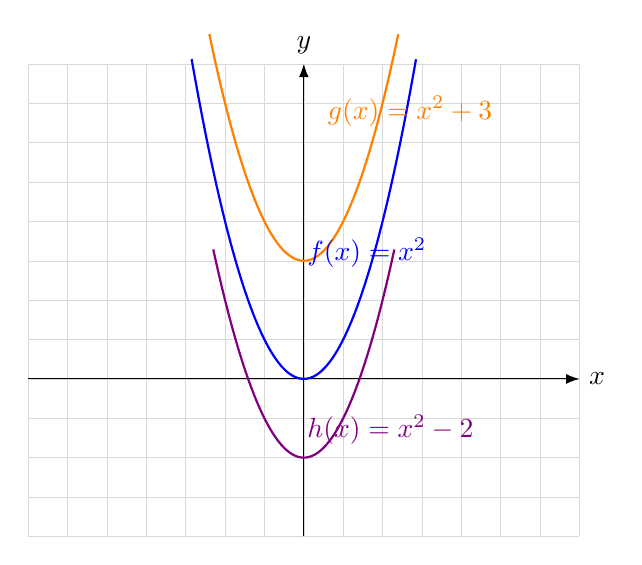
\begin{tikzpicture}[scale=0.5]
\draw[step=1, gray!30, very thin] (-7,-4) grid (7,8);
\draw[-{Latex}] (-7,0) -- (7,0) node[right] {$x$};
\draw[-{Latex}] (0,-4) -- (0,8) node[above] {$y$};
\draw[orange, thick, domain=-2.4:2.4, samples=60, smooth] plot (\x, {\x*\x+3});
\draw[blue, thick, domain=-2.85:2.85, samples=60, smooth] plot (\x, {\x*\x});
\draw[violet, thick, domain=-2.3:2.3, samples=60, smooth] plot (\x, {\x*\x-2});
\node[orange] at (2.7,6.8) {$g(x)=x^2+3$};
\node[blue] at (1.6,3.2) {$f(x)=x^2$};
\node[violet] at (2.2,-1.3) {$h(x)=x^2-2$};
\end{tikzpicture}
\end{center}

\section*{2. Horizontal Shifts}

\begin{friendlyrule}{Horizontal Shifts}
Replacing $x$ by $x+h$ or $x-h$ shifts the graph left or right. If $h$ is a \underline{positive} constant, then
\begin{itemize}
    \item $f(x-h)$ shifts the graph of the function \textbf{right} by $h$ units;
    \item $f(x+h)$ shifts the graph of the function \textbf{left} by $h$ units.
\end{itemize}
\end{friendlyrule}

\begin{center}
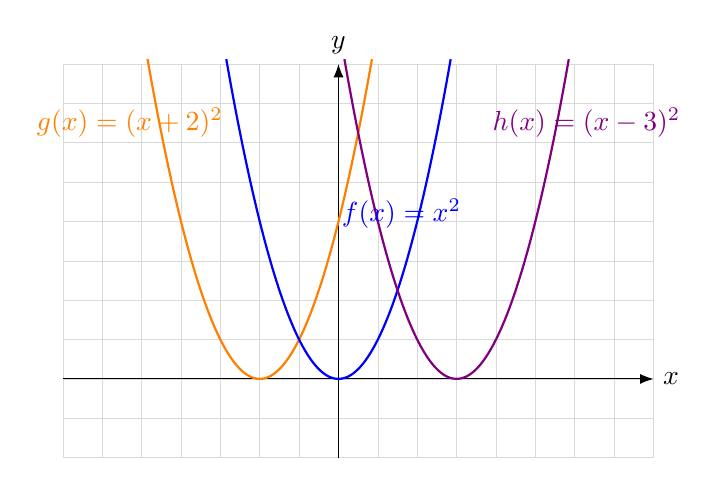
\begin{tikzpicture}[scale=0.5]
\draw[step=1, gray!30, very thin] (-7,-2) grid (8,8);
\draw[-{Latex}] (-7,0) -- (8,0) node[right] {$x$};
\draw[-{Latex}] (0,-2) -- (0,8) node[above] {$y$};
\draw[orange, thick, domain=-4.85:0.85, samples=60, smooth] plot (\x, {(\x+2)*(\x+2)});
\draw[blue, thick, domain=-2.85:2.85, samples=60, smooth] plot (\x, {\x*\x});
\draw[violet, thick, domain=0.15:5.85, samples=60, smooth] plot (\x, {(\x-3)*(\x-3)});
\node[orange] at (-5.3,6.5) {$g(x)=(x+2)^2$};
\node[blue] at (1.6,4.2) {$f(x)=x^2$};
\node[violet] at (6.3,6.5) {$h(x)=(x-3)^2$};
\end{tikzpicture}
\end{center}

\section*{3. Reflecting About the $x$-axis}

\begin{friendlyrule}{Reflecting About the $x$-axis}
Multiplying a function by $-1$ reflects the graph about the $x$-axis.
\end{friendlyrule}

\begin{center}
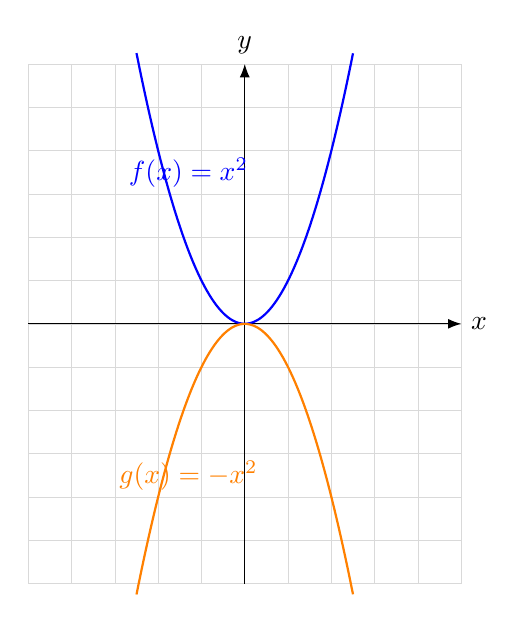
\begin{tikzpicture}[scale=0.55]
\draw[step=1, gray!30, very thin] (-5,-6) grid (5,6);
\draw[-{Latex}] (-5,0) -- (5,0) node[right] {$x$};
\draw[-{Latex}] (0,-6) -- (0,6) node[above] {$y$};
\draw[blue, thick, domain=-2.5:2.5, samples=60, smooth] plot (\x, {\x*\x});
\draw[orange, thick, domain=-2.5:2.5, samples=60, smooth] plot (\x, {-\x*\x});
\node[blue] at (-1.3,3.5) {$f(x)=x^2$};
\node[orange] at (-1.3,-3.5) {$g(x)=-x^2$};
\end{tikzpicture}
\end{center}

\section*{4. Reflecting About the $y$-axis}

\begin{friendlyrule}{Reflecting About the $y$-axis}
Replacing $x$ by $-x$ in the formula for a function reflects the graph about the $y$-axis.
\end{friendlyrule}

\begin{center}
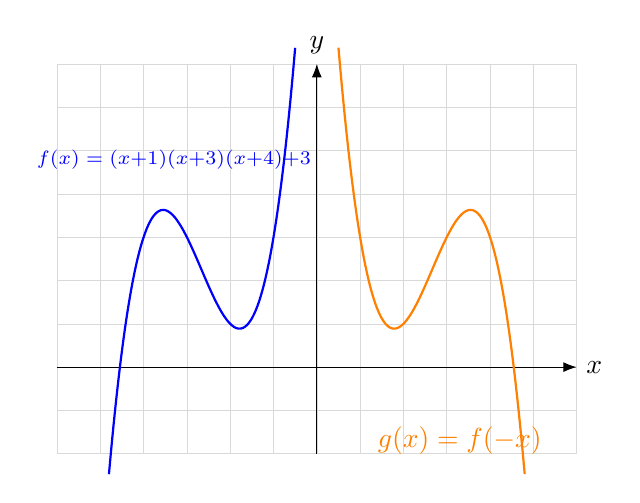
\begin{tikzpicture}[scale=0.55]
\draw[step=1, gray!30, very thin] (-6,-2) grid (6,7);
\draw[-{Latex}] (-6,0) -- (6,0) node[right] {$x$};
\draw[-{Latex}] (0,-2) -- (0,7) node[above] {$y$};
\draw[blue, thick, domain=-4.8:-0.5, samples=80, smooth] plot (\x, {(\x+1)*(\x+3)*(\x+4)+3});
\draw[orange, thick, domain=0.5:4.8, samples=80, smooth] plot (\x, {(-\x+1)*(-\x+3)*(-\x+4)+3});
\node[blue] at (-3.3,4.8) {\scriptsize $f(x)=(x{+}1)(x{+}3)(x{+}4){+}3$};
\node[orange] at (3.3,-1.7) {$g(x)=f(-x)$};
\end{tikzpicture}
\end{center}

\section*{5. Vertical Stretching/Shrinking}

\begin{friendlyrule}{Vertical Stretching/Shrinking}
Multiplying a function by a factor of $a$ \textbf{stretches} (if $a>1$) or \textbf{shrinks} (if $0<a<1$) the graph of the function vertically by a factor of $a$.
\end{friendlyrule}

\begin{center}
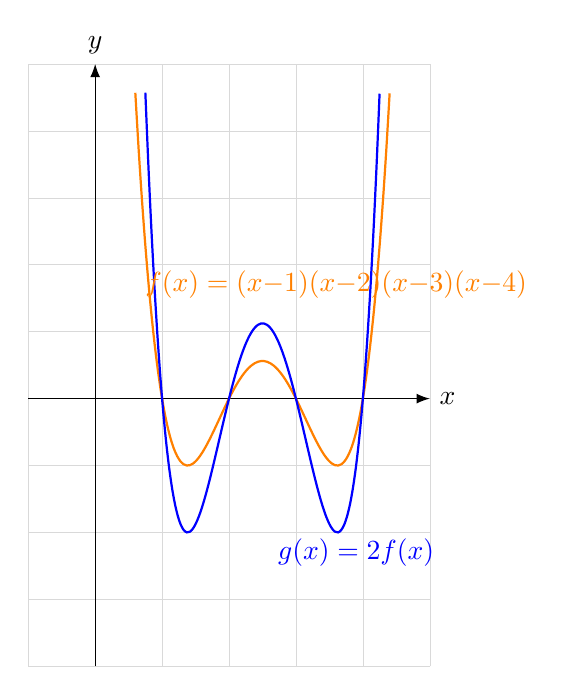
\begin{tikzpicture}[scale=0.85]
\draw[step=1, gray!30, very thin] (-1,-4) grid (5,5);
\draw[-{Latex}] (-1,0) -- (5,0) node[right] {$x$};
\draw[-{Latex}] (0,-4) -- (0,5) node[above] {$y$};
\draw[orange, thick, domain=0.6:4.4, samples=80, smooth] plot (\x, {(\x-1)*(\x-2)*(\x-3)*(\x-4)});
\draw[blue, thick, domain=0.75:4.25, samples=80, smooth] plot (\x, {2*(\x-1)*(\x-2)*(\x-3)*(\x-4)});
\node[orange] at (3.6,1.7) {$f(x)=(x{-}1)(x{-}2)(x{-}3)(x{-}4)$};
\node[blue] at (3.9,-2.3) {$g(x)=2f(x)$};
\end{tikzpicture}
\end{center}

\section*{6. Horizontal Stretching/Shrinking}

\begin{friendlyrule}{Horizontal Stretching/Shrinking}
Multiplying $x$ by a factor of $a$ \textbf{shrinks} (if $0<a<1$) or \textbf{stretches} (if $a>1$) the graph of the function horizontally by a factor of $a$.
\end{friendlyrule}

\begin{center}
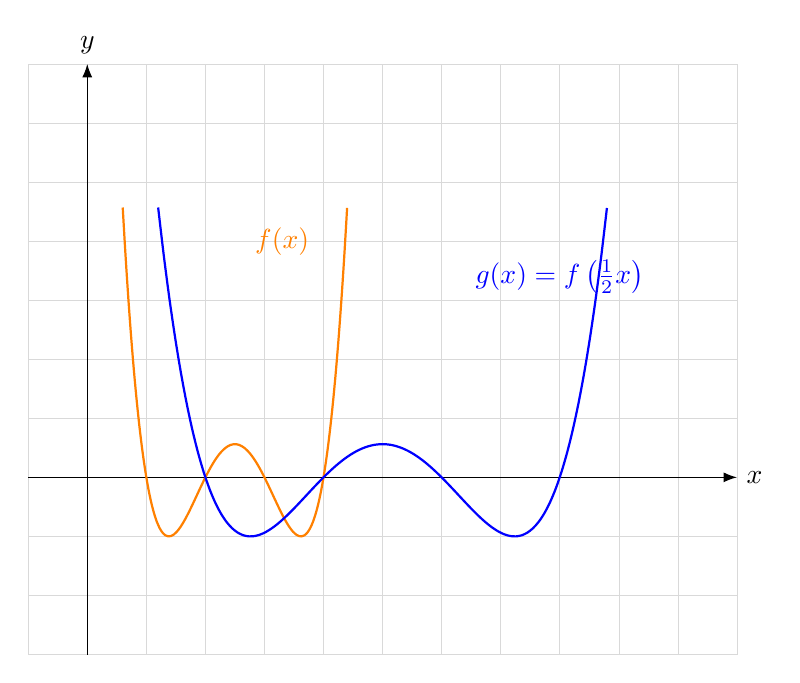
\begin{tikzpicture}[scale=0.75]
\draw[step=1, gray!30, very thin] (-1,-3) grid (11,7);
\draw[-{Latex}] (-1,0) -- (11,0) node[right] {$x$};
\draw[-{Latex}] (0,-3) -- (0,7) node[above] {$y$};
\draw[orange, thick, domain=0.6:4.4, samples=80, smooth] plot (\x, {(\x-1)*(\x-2)*(\x-3)*(\x-4)});
\draw[blue, thick, domain=1.2:8.8, samples=80, smooth] plot (\x, {(0.5*\x-1)*(0.5*\x-2)*(0.5*\x-3)*(0.5*\x-4)});
\node[orange] at (3.3,4) {$f(x)$};
\node[blue] at (8,3.4) {$g(x)=f\left(\frac12 x\right)$};
\end{tikzpicture}
\end{center}

\section*{7. Practice: Sketching Transformations}

\begin{friendlyex}{}
Given the graph of $f(x)=|x|$, sketch the graph of $g(x)=-f(x)-2=-|x|-2$.
\end{friendlyex}

\begin{center}
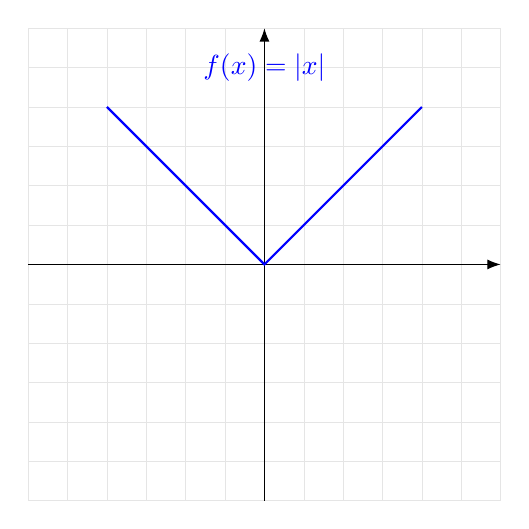
\begin{tikzpicture}[scale=0.5]
\draw[step=1, gray!20, very thin] (-6,-6) grid (6,6);
\draw[-{Latex}] (-6,0) -- (6,0);
\draw[-{Latex}] (0,-6) -- (0,6);
\draw[blue, thick] (-4,4) -- (0,0) -- (4,4);
\node[blue] at (0,5) {$f(x)=|x|$};
\end{tikzpicture}
\end{center}

 

\begin{solutionbox}
$g(x)=-|x|-2$ reflects $f$ about the $x$-axis (the sign flips) and then shifts it down $2$ units. The vertex moves from $(0,0)$ to $(0,-2)$, and the ``V'' now opens \textbf{downward}.

\begin{center}
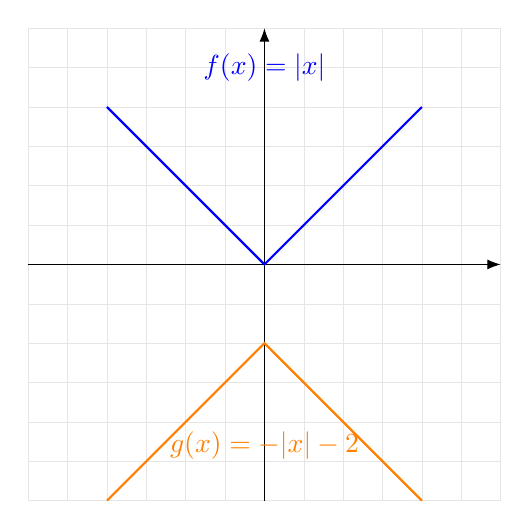
\begin{tikzpicture}[scale=0.5]
\draw[step=1, gray!20, very thin] (-6,-6) grid (6,6);
\draw[-{Latex}] (-6,0) -- (6,0);
\draw[-{Latex}] (0,-6) -- (0,6);
\draw[blue, thick] (-4,4) -- (0,0) -- (4,4);
\draw[orange, thick] (-4,-6) -- (0,-2) -- (4,-6);
\node[blue] at (0,5) {$f(x)=|x|$};
\node[orange] at (0,-4.6) {$g(x)=-|x|-2$};
\end{tikzpicture}
\end{center}
\end{solutionbox}

  

\begin{friendlyex}{}
Given the graph of $f(x)=x^3$, sketch the graph of $g(x)=f(-x)=(-x)^3$.
\end{friendlyex}

\begin{center}
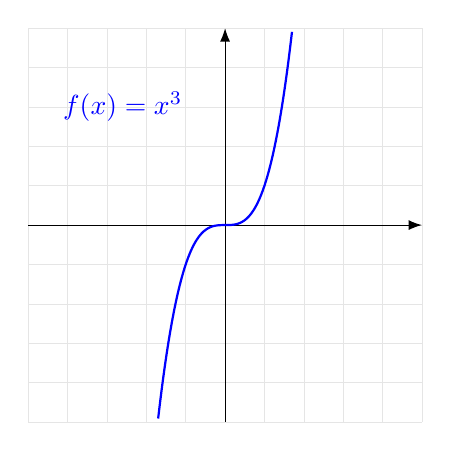
\begin{tikzpicture}[scale=0.5]
\draw[step=1, gray!20, very thin] (-5,-5) grid (5,5);
\draw[-{Latex}] (-5,0) -- (5,0);
\draw[-{Latex}] (0,-5) -- (0,5);
\draw[blue, thick, domain=-1.7:1.7, samples=60, smooth] plot (\x, {\x*\x*\x});
\node[blue] at (-2.6,3) {$f(x)=x^3$};
\end{tikzpicture}
\end{center}

 

\begin{solutionbox}
Since $(-x)^3=-x^3$, we have $g(x)=-x^3$. Reflecting $x^3$ about the $y$-axis gives \textbf{the same picture} as reflecting it about the $x$-axis --- this is a special feature of odd functions like $x^3$.

\begin{center}
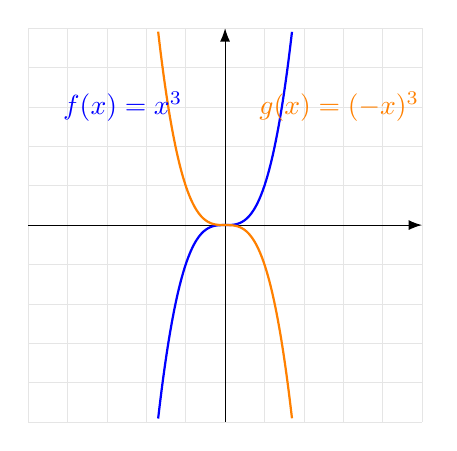
\begin{tikzpicture}[scale=0.5]
\draw[step=1, gray!20, very thin] (-5,-5) grid (5,5);
\draw[-{Latex}] (-5,0) -- (5,0);
\draw[-{Latex}] (0,-5) -- (0,5);
\draw[blue, thick, domain=-1.7:1.7, samples=60, smooth] plot (\x, {\x*\x*\x});
\draw[orange, thick, domain=-1.7:1.7, samples=60, smooth] plot (\x, {-\x*\x*\x});
\node[blue] at (-2.6,3) {$f(x)=x^3$};
\node[orange] at (2.9,3) {$g(x)=(-x)^3$};
\end{tikzpicture}
\end{center}
\end{solutionbox}

  

\begin{friendlyex}{}
Given the graph of $f(x)=x^2$, sketch the graph of $g(x)=(x+2)^2+1$.
\end{friendlyex}

\begin{center}
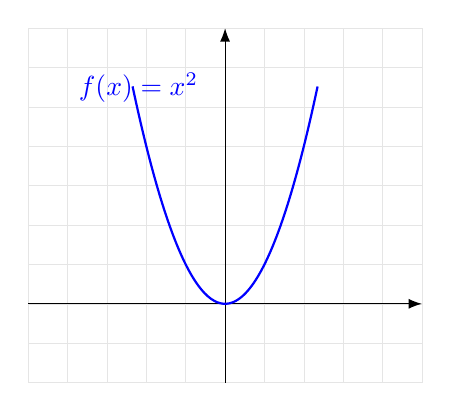
\begin{tikzpicture}[scale=0.5]
\draw[step=1, gray!20, very thin] (-5,-2) grid (5,7);
\draw[-{Latex}] (-5,0) -- (5,0);
\draw[-{Latex}] (0,-2) -- (0,7);
\draw[blue, thick, domain=-2.35:2.35, samples=60, smooth] plot (\x, {\x*\x});
\node[blue] at (-2.2,5.5) {$f(x)=x^2$};
\end{tikzpicture}
\end{center}

 

\begin{solutionbox}
$g(x)=(x+2)^2+1$ shifts $f$ left $2$ units and up $1$ unit. The vertex moves from $(0,0)$ to $(-2,1)$.

\begin{center}
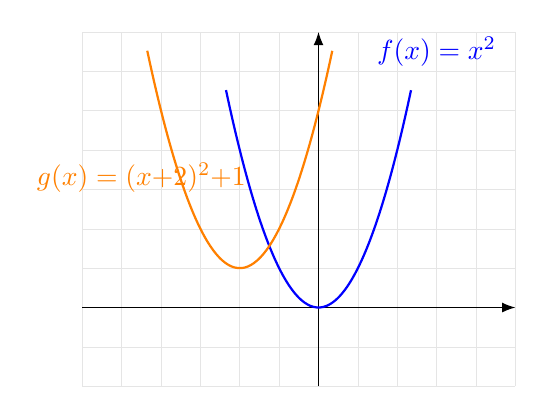
\begin{tikzpicture}[scale=0.5]
\draw[step=1, gray!20, very thin] (-6,-2) grid (5,7);
\draw[-{Latex}] (-6,0) -- (5,0);
\draw[-{Latex}] (0,-2) -- (0,7);
\draw[blue, thick, domain=-2.35:2.35, samples=60, smooth] plot (\x, {\x*\x});
\draw[orange, thick, domain=-4.35:0.35, samples=60, smooth] plot (\x, {(\x+2)*(\x+2)+1});
\node[blue] at (3.0,6.5) {$f(x)=x^2$};
\node[orange] at (-4.5,3.3) {$g(x)=(x{+}2)^2{+}1$};
\end{tikzpicture}
\end{center}
\end{solutionbox}

  

\begin{friendlyex}{}
Starting with the given graph of $f(x)=\sqrt{x}$, sketch the graph of $g(x)=-\sqrt{x}-3$.
\end{friendlyex}

\begin{center}
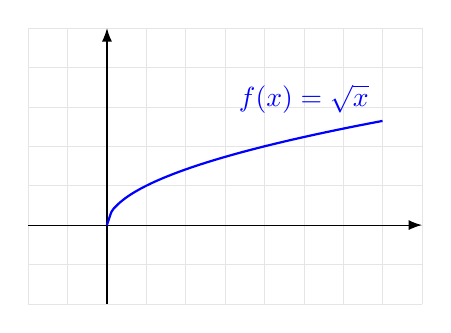
\begin{tikzpicture}[scale=0.5]
\draw[step=1, gray!20, very thin] (-2,-2) grid (8,5);
\draw[-{Latex}] (-2,0) -- (8,0);
\draw[-{Latex}] (0,-2) -- (0,5);
\draw[blue, thick, domain=0:7, samples=60, smooth] plot (\x, {sqrt(\x)});
\node[blue] at (5,3.2) {$f(x)=\sqrt{x}$};
\end{tikzpicture}
\end{center}

 

\begin{solutionbox}
$g(x)=-\sqrt{x}-3$ reflects $f$ about the $x$-axis and then shifts it down $3$ units.

\begin{center}
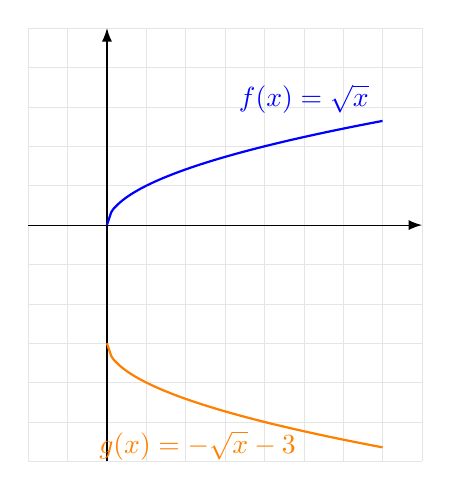
\begin{tikzpicture}[scale=0.5]
\draw[step=1, gray!20, very thin] (-2,-6) grid (8,5);
\draw[-{Latex}] (-2,0) -- (8,0);
\draw[-{Latex}] (0,-6) -- (0,5);
\draw[blue, thick, domain=0:7, samples=60, smooth] plot (\x, {sqrt(\x)});
\draw[orange, thick, domain=0:7, samples=60, smooth] plot (\x, {-sqrt(\x)-3});
\node[blue] at (5,3.2) {$f(x)=\sqrt{x}$};
\node[orange] at (2.3,-5.6) {$g(x)=-\sqrt{x}-3$};
\end{tikzpicture}
\end{center}
\end{solutionbox}

  

\section*{8. Describing Combinations of Transformations}

\begin{friendlyex}{}
List all the transformations that have been applied to $y=f(x)$ to obtain $y=\dfrac14 f(x+2)-5$.
\end{friendlyex}

 

\begin{solutionbox}
Reading from the inside out:
\begin{itemize}
    \item $f(x+2)$: shift \textbf{left} $2$ units;
    \item $\dfrac14 f(x+2)$: vertically \textbf{shrink} by a factor of $\dfrac14$;
    \item $\dfrac14 f(x+2)-5$: shift \textbf{down} $5$ units.
\end{itemize}
\end{solutionbox}

  

\begin{friendlyex}{}
List all the transformations that have been applied to $y=f(x)$ to obtain $g(x)=3f(-x+1)+2$.
\end{friendlyex}

 

\begin{solutionbox}
Rewrite the argument: $-x+1=-(x-1)$, so $g(x)=3f(-(x-1))+2$.
\begin{itemize}
    \item $f(-x)$: reflect about the \textbf{$y$-axis};
    \item $f(-(x-1))$: shift \textbf{right} $1$ unit;
    \item $3f(-(x-1))$: vertically \textbf{stretch} by a factor of $3$;
    \item $3f(-(x-1))+2$: shift \textbf{up} $2$ units.
\end{itemize}
\end{solutionbox}

  

\begin{friendlyex}{}
Describe all the transformations that have been applied to $y=f(x)$ to obtain $y=-2f(-(x+4))-7$.
\end{friendlyex}

 

\begin{solutionbox}
\begin{itemize}
    \item $f(-x)$: reflect about the \textbf{$y$-axis};
    \item $f(-(x+4))$: shift \textbf{left} $4$ units;
    \item $-2f(-(x+4))$: vertically \textbf{stretch} by a factor of $2$ and reflect about the \textbf{$x$-axis};
    \item $-2f(-(x+4))-7$: shift \textbf{down} $7$ units.
\end{itemize}
\end{solutionbox}

  

\begin{friendlyex}{}
Write a formula for the function obtained when the graph of $f(x)=\sqrt{x}$ is shifted up $2$ units, shifted left $3$ units, and reflected across the $x$-axis.
\end{friendlyex}

 

\begin{solutionbox}
Apply the transformations in the order listed:

\[
\sqrt{x}\ \xrightarrow{\text{up }2}\ \sqrt{x}+2\ \xrightarrow{\text{left }3}\ \sqrt{x+3}+2\ \xrightarrow{\text{reflect across }x\text{-axis}}\ -\left(\sqrt{x+3}+2\right).
\]

\[
g(x)=-\sqrt{x+3}-2.
\]
\end{solutionbox}

  

\begin{friendlyex}{}
Write a formula for the function obtained when the graph of $f(x)=\dfrac{1}{\sin(x)}$ is stretched horizontally by $3$, reflected across the $y$-axis, and moved down $2$ units.
\end{friendlyex}

 

\begin{solutionbox}
Apply the transformations in the order listed:

\[
\frac{1}{\sin x}\ \xrightarrow{\text{stretch horiz. by }3}\ \frac{1}{\sin(x/3)}\ \xrightarrow{\text{reflect across }y\text{-axis}}\ \frac{1}{\sin(-x/3)},
\]

\[
\frac{1}{\sin(-x/3)}\ \xrightarrow{\text{down }2}\ \frac{1}{\sin(-x/3)}-2.
\]

Since $\sin(-x/3)=-\sin(x/3)$, this simplifies to

\[
g(x)=-\frac{1}{\sin(x/3)}-2.
\]
\end{solutionbox}

  

\section*{Summary}

\begin{friendlyrule}{Key Ideas}
\begin{itemize}
    \item $f(x)+k$ / $f(x)-k$: shift up/down by $k$.
    \item $f(x-h)$ / $f(x+h)$: shift right/left by $h$.
    \item $-f(x)$: reflect about the $x$-axis. $f(-x)$: reflect about the $y$-axis.
    \item $a\cdot f(x)$: vertical stretch ($a>1$) or shrink ($0<a<1$).
    \item $f(ax)$: horizontal shrink ($a>1$) or stretch ($0<a<1$).
    \item When combining transformations, work from the inside of the formula outward, and build new formulas by applying each transformation to the previous result, in the order given.
\end{itemize}
\end{friendlyrule}

\end{document}
